\begin{figure}
  \centering
  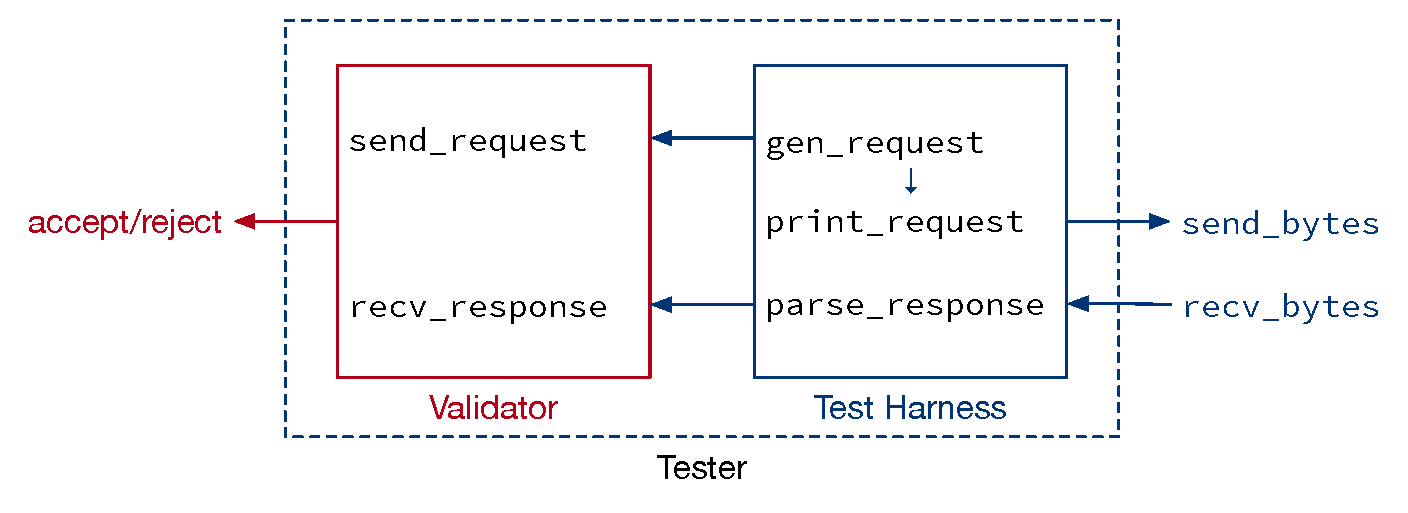
\includegraphics[width=.9\textwidth]{figures/harness-outline}
  \caption{Tester architecture outline.}
  \label{fig:overview}
\end{figure}

This section introduces the abstract architecture of an interactive tester,
using the networked server as an example.  I'll present a na\"ive implementation
of the test harness, which will be improved in the following sections.

The test harness interacts with the environment and provides the observations
for the validator.  The validator may represent requests and responses as
abstract datatypes for the convenience of specification.  The test harness
translates these abstract representations into bytes transmitted on the
underlying channel.

As shown in \autoref{fig:overview}, when the validator wants to observe a sent
request, the harness generates the request and encodes it into bytes to send.
Conversely, when the validator wants to observe a received response, the harness
receives bytes from the environment and decodes them into abstract messages.

\begin{figure}
\begin{lstlisting}[numbers=left]
Definition gen_packet: IO concrete_packet :=
  src          <- random_conn;;
  method       <- oneof [Get; Put];;
  target       <- random_path;;%\label{line:random-path}%
  precondition <- oneof [IfMatch, IfNoneMatch];;
  etag         <- random_etag;;
  payload      <- random_string;;
  ret { Source      := src;
        Destination := server_conn;
        Data        := inr { Method     := method;
                             TargetPath := target;
                             Headers    := [(precondition, etag)];
                             Payload    := payload
                           }
      }.
\end{lstlisting}
\caption{Na\"ive generator for HTTP requests.}
\label{fig:naive-generator}
\end{figure}

A generator is a randomized program that produces test inputs.  One example is
the \ilc{gen_packet} function in \autoref{fig:execute}.  The HTTP packet
generator can be na\"ively implementation as shown in
\autoref{fig:naive-generator}.  It fills in the request's fields with arbitrary
values, and has limited coverage of the SUT's behavior.  This is because the
request target and ETags are both generated randomly, but a request is
interesting only if its ETag matches its target's corresponding resource stored
on the server.  A randomly generated request would result in 404 Not Found and
412 Precondition Failed in almost all cases.

To reveal more interesting behavior from the SUT, we should tune the generator's
distribution to emphasize certain patterns of the test input.  For example, if
the tester knows the set of paths where the server has stored resources, then it
can generate more paths within the set to hit the existing resources; if the
tester has observed some ETags generated by the server, then it can include
these ETags in future requests.  In the next section, I'll explain how to
implement such heuristics in ITree-based testers.
